\documentclass[10pt]{beamer}

\usetheme{Oxygen}
\usepackage{thumbpdf}
\usepackage{wasysym}
\usepackage{ucs}
\usepackage[utf8]{inputenc}
\usepackage{pgf,pgfarrows,pgfnodes,pgfautomata,pgfheaps,pgfshade}
\usepackage{verbatim}


\usepackage{ragged2e} % maneja la alineación del documento
\usepackage[spanish]{babel} % Títulos en español
\usepackage[utf8]{inputenc}
%\usepackage[latin1]{inputenc} % Caracteres con acentos.
\usepackage{graphicx} % Soporte para gráficos
\usepackage[none]{hyphenat} % indica a LaTeX que no debe hacer partición de palabras
\usepackage[T1]{fontenc} % manejo de fuentes
\usepackage{array}
\usepackage{amsmath}
\usepackage{amssymb}
\usepackage{float}
\usepackage{ra  gged2e}
\usepackage [all]{xy}
\usepackage{lmodern}
\usepackage{multirow}
\usepackage{multicol}
\usepackage{tikz}

\setbeamersize{text margin left=9mm,text margin right=7mm} 


\pdfinfo
{
  /Title       (TD)
  /Creator     (TeX)
  /Author      (Orlando Joaqui Barandica)
}


\title{Maestría en Analítica e Inteligencia de Negocios}
\subtitle{Tema: Logit}
\author{PhD. Orlando Joaqui Barandica} 
\institute{Universidad del Valle}
\date{2022}

\sloppy % Indica a LaTex que debe minimizar el corte de las palabras para pasar de una línea a otra
\justifying % justificar todo el documento


\begin{document}

\frame{\titlepage}


\begin{frame}
  \frametitle{Contenido}
  \tableofcontents[hidesubsections]
\end{frame}

\AtBeginSection[]
{
  \frame<handout:0>
  {
    \frametitle{Contenido}
    \tableofcontents[currentsection,hideallsubsections]
  }
}

    
\AtBeginSubsection[]
{
  \frame<handout:0>
  {
    \frametitle{Contenido}
    \tableofcontents[sectionstyle=show/hide,subsectionstyle=show/shaded/hide]
  }
}

\newcommand<>{\highlighton}[1]{%
  \alt#2{\structure{#1}}{{#1}}
}

\newcommand{\icon}[1]{\pgfimage[height=1em]{#1}}



%%%%%%%%%%%%%%%%%%%%%%%%%%%%%%%%%%%%%%%%%
%%%%%%%%%% Content starts here %%%%%%%%%%
%%%%%%%%%%%%%%%%%%%%%%%%%%%%%%%%%%%%%%%%%


\section{Modelos variable dependiente cualitativa}
\begin{frame}
\frametitle{Modelos variable dependiente cualitativa}



Se consideran modelos de regresión en los que la variable dependiente puede ser una variable de tipo cualitativo: BINARIA, ORDINAL, NOMINAL o puede tratarse de una variable de CONTEO. 
\vspace{4mm}

\begin{itemize}

\item \textbf{Variable binaria:} Tiene dos categorías. Normalmente indica que ha ocurrido un suceso, que alguna característica está presente o que se elige una opción. 

\item Ejemplos: Actividad laboral; Compra de un producto; Participación en las elecciones ...
\end{itemize}




\end{frame}


%%%%%%%%%%%%%%%%%%%%%%%%%%%%%%%%%%%%%%%%%%%%%%%%%%%%%%%%%%%%


\begin{frame}
\frametitle{Modelos variable dependiente cualitativa}



\begin{itemize}

\item \textbf{Variable ordinal:} Tienen categorías que pueden ordenarse en forma ascendente o descendente. 

\item Ejemplo: Nivel de aceptación respecto a una afirmación, con respuestas: \\
``completamente de acuerdo'', ``de acuerdo'', ``en desacuerdo'', ``completamente en desacuerdo'' \\
\vspace{4mm}
Valoración del nivel de satisfacción de un bien o servicio (``muy satisfecho'',..., ``muy insatisfecho'')\\
\vspace{4mm}
Frecuencia de una determinada acción (``nunca'',..., ``muy frecuentemente'); Nivel de educación alcanzado; ...
\end{itemize}




\end{frame}


%%%%%%%%%%%%%%%%%%%%%%%%%%%%%%%%%%%%%%%%%%%%%%%%%%%%%%%%%%%%



\begin{frame}
\frametitle{Modelos variable dependiente cualitativa}



\begin{itemize}

\item \textbf{Variable nominal:} Variable con múltiples respuestas que no siguen un orden predeterminado. 

\item Ejemplos: Rama de actividad laboral; Estatus matrimonial; Elección política; Preferencia de marcas, ...

\end{itemize}

\end{frame}


%%%%%%%%%%%%%%%%%%%%%%%%%%%%%%%%%%%%%%%%%%%%%%%%%%%%%%%%%%%%



\begin{frame}
\frametitle{Modelos variable dependiente cualitativa}


\begin{figure}
\begin{center}
    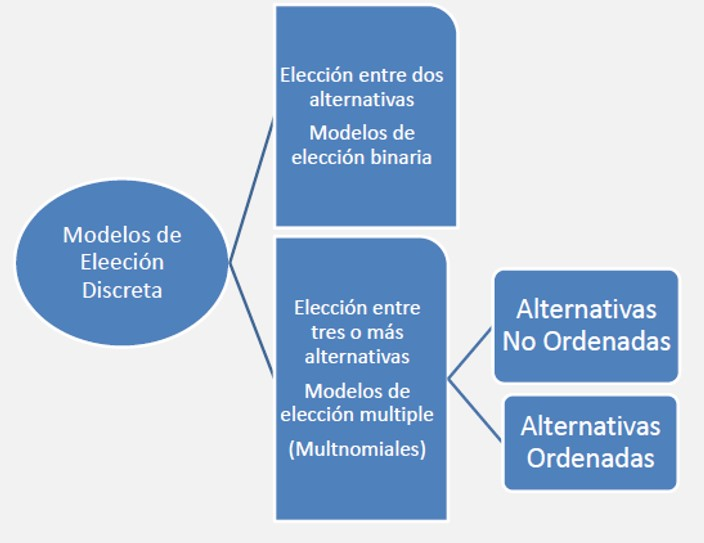
\includegraphics[width=0.6\textwidth]{9_1.JPG}
\end{center}
\end{figure}

\end{frame}


%%%%%%%%%%%%%%%%%%%%%%%%%%%%%%%%%%%%%%%%%%%%%%%%%%%%%%%%%%%%




\begin{frame}
\frametitle{Modelos variable dependiente cualitativa}


Los modelos de elección discreta resultan apropiados cuando el objetivo no es predecir el comportamiento medio de un agregado, sino analizar los factores determinantes de la \highlighton{probabilidad} de que un agente económico individual elija un curso de acción dentro de un conjunto, generalmente finito, de opciones posibles. 

\vspace{4mm}
\begin{itemize}
\item $Y$ cuantitativa: $E(Y_i | X_{1i}, X_{2i}, ..., X_{ki} )$

\vspace{3mm}

\item $Y$ cualitativa: Probabilidad de que suceda el evento de interés.

\end{itemize}


\end{frame}


%%%%%%%%%%%%%%%%%%%%%%%%%%%%%%%%%%%%%%%%%%%%%%%%%%%%%%%%%%%%




\begin{frame}
\frametitle{Modelos de respuesta binaria}


Hay cuatro métodos para crear un modelo de probabilidad para una variable de respuesta binaria:

\begin{enumerate}
\item El modelo lineal de probabilidad (MLP)
\item El modelo logit
\item El modelo probit
\item El modelo tobit
\end{enumerate}


\end{frame}


%%%%%%%%%%%%%%%%%%%%%%%%%%%%%%%%%%%%%%%%%%%%%%%%%%%%%%%%%%%%


\section{MLP}
\begin{frame}
\frametitle{Modelo lineal de probabilidad (MLP)}


Considere el siguiente modelo simple:

\begin{equation}
Y = \beta_0 +\beta_1 X + u
\end{equation}

\textit{donde X = el ingreso familiar, y Y = 1 si la familia tiene casa propia y 0 si la familia no tiene casa propia.}\\
\vspace{4mm}
Parece un modelo de regresión lineal común, pero debido a que la variable regresada es binaria, o dicótoma, se denomina modelo lineal de probabilidad (MLP).\\
\vspace{4mm}

\textbf{La expectativa condicional de que $Y$ dado $X$, \highlighton{$E(Y/X)$} puede interpretarse como la probabilidad condicional de que el suceso tenga lugar dado $X$, es decir: \highlighton{$P(Y=1|X)$}
}
\end{frame}


%%%%%%%%%%%%%%%%%%%%%%%%%%%%%%%%%%%%%%%%%%%%%%%%%%%%%%%%%%%%





\begin{frame}
\frametitle{Modelo lineal de probabilidad (MLP)}


En el MLP, la variable dependiente toma únicamente dos valores:
	

\begin{equation}
Y_i = \left\lbrace
\begin{matrix} 
1 & \mbox{si ocurre un evento determinado} \\ 
0 & \mbox{si el evento no ocurre}
\end{matrix}
\right.
\end{equation}

El valor esperado de esta variable, puede interpretarse como la probabilidad de que ocurra el evento:  

\begin{equation}
E(Y_i/X_i) = 1 * Pr(Y_i = 1|X_i) + 0 * Pr(Y_i = 0|X_i)
\end{equation}

\vspace{4mm}

El valor esperado de $Y_i$ dado $X$ es la probabilidad de que $Y_i = 1$. Por tanto, el modelo de probabilidad lineal se puede escribir como: \textit{(Asumiendo que $E(u_i) = 0$ para obtener estimadores insesgados)}

\begin{equation}
p_i = Pr(Y_i = 1|X_i) =  \beta_0 +\beta_1 X
\end{equation}

\end{frame}


%%%%%%%%%%%%%%%%%%%%%%%%%%%%%%%%%%%%%%%%%%%%%%%%%%%%%%%%%%%%


\begin{frame}
\frametitle{Problemas de MLP}


Los problemas se presentan como consecuencia de que la ``nube de puntos'' a partir de la cual se debe ajustar la recta de regresión es en este caso un par de líneas paralelas sobre los dos únicos valores de la dependiente. 


\begin{figure}
\begin{center}
    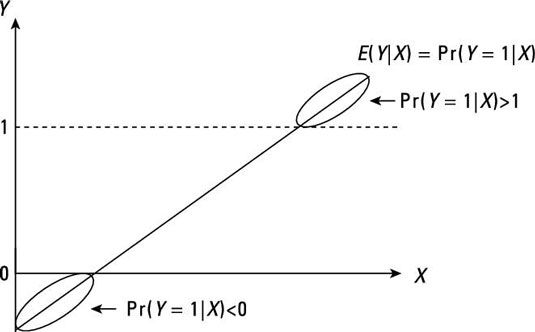
\includegraphics[width=0.6\textwidth]{9_2.JPG}
\end{center}
\end{figure}



\end{frame}


%%%%%%%%%%%%%%%%%%%%%%%%%%%%%%%%%%%%%%%%%%%%%%%%%%%%%%%%%%%%



\begin{frame}
\frametitle{Problemas de MLP}


\textbf{No normalidad de las perturbaciones:} Problema que no afecta la insesgadez de los estimadores puntuales, aunque el proceso de inferencia basado en una distribución normal sólo será válido si la muestra es lo suficientemente grande. 

\vspace{4mm}

\textbf{Heterocedasticidad del término de perturbación:} Por tanto, los estimadores MCO son menos eficientes. 



\end{frame}


%%%%%%%%%%%%%%%%%%%%%%%%%%%%%%%%%%%%%%%%%%%%%%%%%%%%%%%%%%%%



\begin{frame}
\frametitle{Problemas de MLP}


\textbf{Probabilidades predichas inconsistentes:} no es posible garantizar que estén acotadas entre 0 y 1. 

\vspace{4mm}

\textbf{Interpretación de los coeficientes:} El modelo supone que el efecto de las variables sobre la probabilidad es constante y lineal en todo el recorrido de las variables. 

\vspace{4mm}

\textbf{El Coeficiente de determinación:} No es apropiado. 



\end{frame}


%%%%%%%%%%%%%%%%%%%%%%%%%%%%%%%%%%%%%%%%%%%%%%%%%%%%%%%%%%%%



\begin{frame}
\frametitle{Problemas de MLP}


\textbf{Alternativa al modelo lineal de probabilidad}

\vspace{4mm}

Interesa un modelo que reproduzca adecuadamente el comportamiento de una función de probabilidad. 

\vspace{4mm}

La \highlighton{$Pr(Y_i = 1|X_i)$}, deberá especificarse para que no supere los límites de 0 y 1, y con efectos no lineales de las variables explicativas: 


\begin{figure}
\begin{center}
    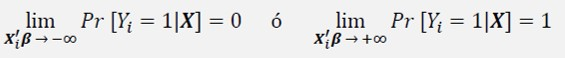
\includegraphics[width=0.6\textwidth]{9_3.JPG}
\end{center}
\end{figure}


\end{frame}


%%%%%%%%%%%%%%%%%%%%%%%%%%%%%%%%%%%%%%%%%%%%%%%%%%%%%%%%%%%%





\begin{frame}
\frametitle{Modelo de elección binaria}


Para modelar este comportamiento, las distribuciones más empleadas han sido la normal estándar y la logística. 

\vspace{4mm}

Cuando se emplea como función de probabilidad la distribución normal, se obtiene el denominado modelo \textbf{Probit}, mientras que la distribución logística proporciona el modelo \textbf{Logit}. 

\begin{figure}
\begin{center}
    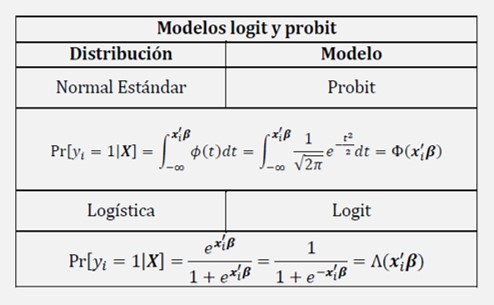
\includegraphics[width=0.6\textwidth]{9_4.JPG}
\end{center}
\end{figure}


\end{frame}


%%%%%%%%%%%%%%%%%%%%%%%%%%%%%%%%%%%%%%%%%%%%%%%%%%%%%%%%%%%%



\section{Logit}
\begin{frame}
\frametitle{Modelo Logit}


Ejemplo: 

\begin{equation}
P_i = \beta_0 +\beta_1 X + u
\end{equation}

$X$ es el ingreso y \highlighton{$Pr(Y_i = 1|X_i)$} significa que la familia es propietaria de una casa.

\vspace{4mm}

Pero considere ahora la siguiente representación de la propiedad de vivienda:

\begin{equation}
P_i = \frac{1}{1 + e^{-(\beta_0 + \beta_1 X)}}
\end{equation}

\begin{equation}
P_i = \frac{1}{1 + e^{-Z}} \quad \quad \mbox{Donde:}  \quad Z = \beta_0 + \beta_1 X
\end{equation}

\begin{equation}
P_i = \frac{1}{1 + e^{-Z}} = \frac{e^Z}{1 + e^Z} \Longrightarrow \highlighton{\textbf{Función de distribución logística}}
\end{equation}


\end{frame}


%%%%%%%%%%%%%%%%%%%%%%%%%%%%%%%%%%%%%%%%%%%%%%%%%%%%%%%%%%%%




\begin{frame}
\frametitle{Modelo Logit}

$P_i$ es no lineal no sólo en $X$ sino también en las $\beta_i$. Esto significa que no podemos estimar los parámetros con el procedimiento habitual de MCO.


\vspace{4mm}

\textbf{Es necesario linealizar a $P_i$}

\vspace{4mm}

Si $P_i$ es la probabilidad de tener casa propia, entonces $(1 - P_i)$, es la probabilidad de no tener casa propia.


\begin{equation}
1 - P_i = \frac{1}{1 + e^{Z}}
\end{equation}

\vspace{4mm}

Por consiguiente, podemos escribir

\begin{equation}
\frac{P_i}{1 - P_i} = \frac{1 + e^{Z}}{1 + e^{-Z}} = e^{Z}
\end{equation}



\end{frame}


%%%%%%%%%%%%%%%%%%%%%%%%%%%%%%%%%%%%%%%%%%%%%%%%%%%%%%%%%%%%



\begin{frame}
\frametitle{Modelo Logit}

\begin{equation}
\frac{P_i}{1 - P_i}
\end{equation}

\vspace{4mm}

Es la razón de las probabilidades en favor de tener una casa propia: la razón de la probabilidad de que una familia posea una casa propia respecto de la probabilidad de que no la posea. 

\vspace{4mm}

\textbf{Ahora si se aplica logaritmo natural sea $L$}

\vspace{4mm}

\begin{eqnarray}
L = ln \left(  \frac{P_i}{1 - P_i} \right)  = ln (e^{Z}) & = & Z \\
 & = &  \beta_0 + \beta_1 X
\end{eqnarray}

De ahí se tiene entonces el modelo logit.
\end{frame}


%%%%%%%%%%%%%%%%%%%%%%%%%%%%%%%%%%%%%%%%%%%%%%%%%%%%%%%%%%%%



\begin{frame}
\frametitle{Modelo Logit}

\textbf{Características del modelo logit:}

\vspace{4mm}

\begin{itemize}
\item P va de 0 a 1. \\

\item Aunque $L$ es lineal en $X$, las probabilidades en sí mismas no lo son. Esta propiedad contrasta con el MLP.

\item Se pueden añadir tantas regresoras como indique la teoría subyacente.

\item Los modelos logit se estiman usualmente empleando el \highlighton{método de máxima verosimilitud (MV).}

\item Como empleamos MV, que en general es para muestras grandes, los errores estándar estimados son asintóticos. 

\item Como resultado, en vez del estadístico t para evaluar la importancia estadística de un coeficiente, empleamos el estadístico (normal estandarizado) \textbf{Z}

\end{itemize}


\end{frame}


%%%%%%%%%%%%%%%%%%%%%%%%%%%%%%%%%%%%%%%%%%%%%%%%%%%%%%%%%%%%



\begin{frame}
\frametitle{Modelo Logit}

\textbf{Características del modelo logit:}

\vspace{4mm}

\begin{itemize}
\item La medida convencional de la bondad de ajuste, $R^2$, no es particularmente significativa para los modelos con regresada binaria. Se pueden utilizar similares:

\vspace{4mm}

\begin{itemize}
\item pseudo $R^2$
\item $R^2$ McFadden
\item cuenta $R^2$


\end{itemize}

\end{itemize}

\begin{equation}
\mbox{Cuenta } R^2 = \frac{\mbox{Número de predicciones correctas}}{\mbox{Número total de observaciones}}
\end{equation}
\vspace{4mm}

Como $Y$ en el modelo logit toma el valor de 1 o de 0, si la probabilidad pronosticada es mayor que 0.5, se clasifica como si fuese 1, pero si es menor que dicho valor, se considera 0. Así, se cuenta el número de predicciones correctas y se calcula $R^2$

\end{frame}


%%%%%%%%%%%%%%%%%%%%%%%%%%%%%%%%%%%%%%%%%%%%%%%%%%%%%%%%%%%%








%%%%%%%%%%%%%%%%%%%%%%%%%%%%%%%%%%%%%%%%%%%%%%%%%%%%%%%%%%%%




\begin{frame}
\frametitle{Ejemplo}

\begin{figure}
\begin{center}
    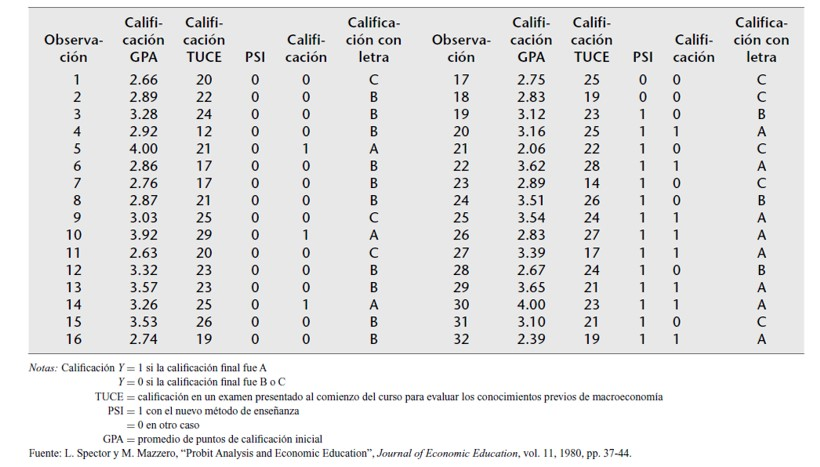
\includegraphics[width=0.9\textwidth]{9_5.JPG}
\end{center}
\end{figure}


\end{frame}

%%%%%%%%%%%%%%%%%%%%%%%%%%%%%%%%%%%%%%%%%%%%%%%%%%%%%%%%%%%%



\begin{frame}
\frametitle{Ejemplo}

Sea \highlighton{Y = 1}, si la calificación final de un estudiante en un curso intermedio de microeconomía fue A, y \highlighton{Y = 0} si esa calificación final fue B o C. Spector y Mazzeo utilizaron el GPA (promedio de puntos de calificación), TUCE y PSI (Sistema de Enseñanza Personalizada) de Estados Unidos como predictores de la calificación. El modelo logit en este caso se expresa como:

\vspace{4mm}

\begin{equation}
ln \left(  \frac{P_i}{1 - P_i} \right) = \beta_0 + \beta_1 GPA + \beta_2 TUCE + \beta_3 PSI + u
\end{equation}


\end{frame}

%%%%%%%%%%%%%%%%%%%%%%%%%%%%%%%%%%%%%%%%%%%%%%%%%%%%%%%%%%%%



\begin{frame}
\frametitle{Ejemplo}

El comando en Stata es \textbf{logit}

\pause
\vspace{4mm}

\textit{\textbf{logit Calificacion GPA TUCE PSI}}

\pause

\begin{figure}
\begin{center}
    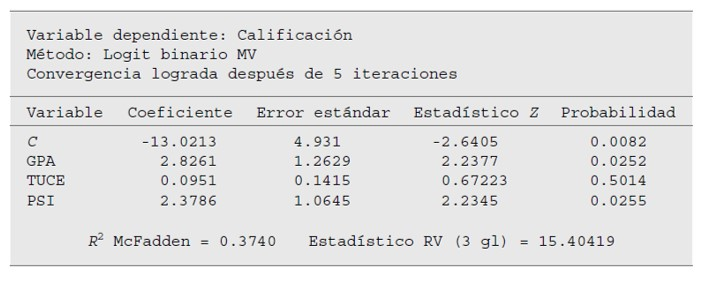
\includegraphics[width=0.9\textwidth]{9_6.JPG}
\end{center}
\end{figure}


\end{frame}

%%%%%%%%%%%%%%%%%%%%%%%%%%%%%%%%%%%%%%%%%%%%%%%%%%%%%%%%%%%%




\begin{frame}
\frametitle{Ejemplo}

\begin{figure}
\begin{center}
    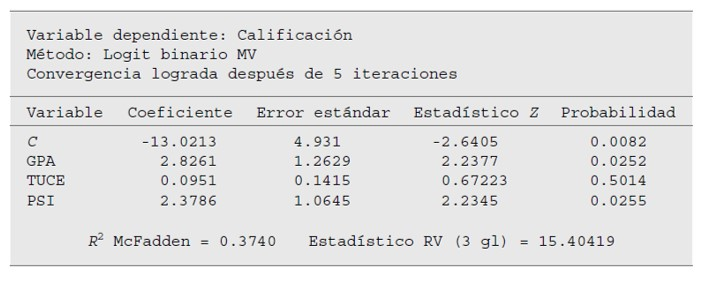
\includegraphics[width=0.8\textwidth]{9_6.JPG}
\end{center}
\end{figure}


\textbf{Interpretaciones:}

\vspace{4mm}
Cada coeficiente de pendiente es un coeficiente de pendiente parcial y mide el cambio en el logit estimado correspondiente a una unidad de cambio del valor de la regresada dada (con las demás regresoras constantes).


\end{frame}

%%%%%%%%%%%%%%%%%%%%%%%%%%%%%%%%%%%%%%%%%%%%%%%%%%%%%%%%%%%%



\begin{frame}
\frametitle{Ejemplo}

\begin{figure}
\begin{center}
    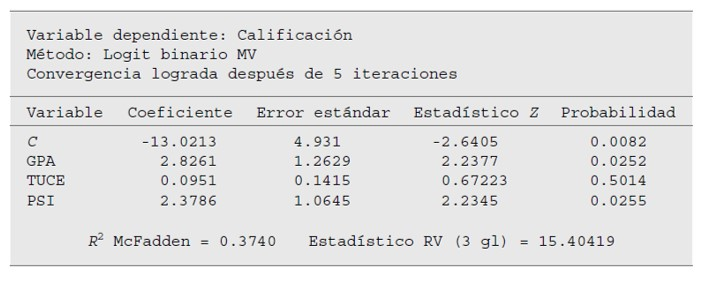
\includegraphics[width=0.8\textwidth]{9_6.JPG}
\end{center}
\end{figure}


\textbf{Interpretaciones:} Ejemplo

\vspace{4mm}
El coeficiente del GPA igual a 2.8261 significa que, mientras las
demás variables se mantengan constantes, si el GPA se incrementa en una unidad, en promedio el logit estimado aumenta casi 2.83 unidades, lo cual indica una relación positiva entre ambos.


\end{frame}

%%%%%%%%%%%%%%%%%%%%%%%%%%%%%%%%%%%%%%%%%%%%%%%%%%%%%%%%%%%%



\begin{frame}
\frametitle{Ejemplo}

\begin{figure}
\begin{center}
    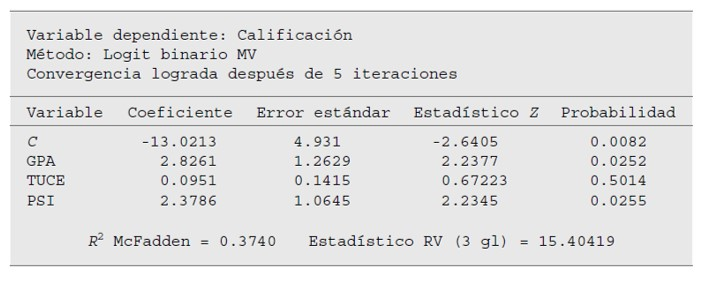
\includegraphics[width=0.8\textwidth]{9_6.JPG}
\end{center}
\end{figure}


\textbf{Interpretaciones:} Ejemplo \textit{``Posibilidad''}

\vspace{4mm}
Una interpretación más significativa se da en términos de las posibilidades en favor, las cuales se obtienen al tomar el antilogaritmo de los diversos coeficientes.


\end{frame}

%%%%%%%%%%%%%%%%%%%%%%%%%%%%%%%%%%%%%%%%%%%%%%%%%%%%%%%%%%%%



\begin{frame}
\frametitle{Ejemplo}

\begin{figure}
\begin{center}
    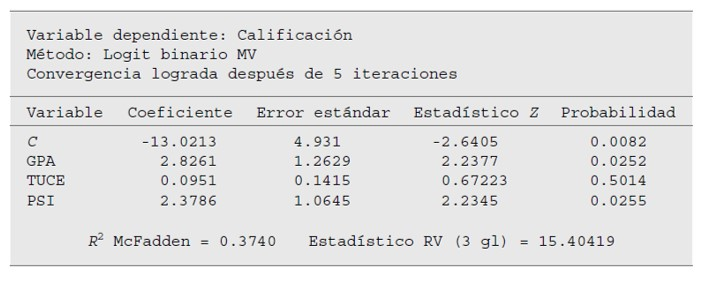
\includegraphics[width=0.8\textwidth]{9_6.JPG}
\end{center}
\end{figure}


\textbf{Interpretaciones:} Ejemplo \textit{``Posibilidad''}

\vspace{3mm}
\highlighton{El antilogaritmo de PSI: 10.7897 $(\approx e^{2.3786})$.\\}

Esto indica que los estudiantes expuestos al nuevo método de enseñanza son por encima de 10 veces más propensos a obtener una A que quienes no están expuestos al nuevo método, en tanto no cambien los demás factores.

\end{frame}

%%%%%%%%%%%%%%%%%%%%%%%%%%%%%%%%%%%%%%%%%%%%%%%%%%%%%%%%%%%%





\begin{frame}
\frametitle{Ejemplo}

\textbf{Interpretaciones:} Ejemplo \textit{``Probabilidad''}

\vspace{3mm}
los coeficientes de pendiente no dan la tasa de cambio de la probabilidad por cada unidad de cambio en la regresora. Es necesario calcularlos: \highlighton{Efectos marginales: dy/dx}

\vspace{3mm}

Comando en Stata: \textbf{mfx}

\end{frame}

%%%%%%%%%%%%%%%%%%%%%%%%%%%%%%%%%%%%%%%%%%%%%%%%%%%%%%%%%%%%




\section{Probit}
\begin{frame}
\frametitle{Modelo Probit}

Para explicar el comportamiento de una variable dependiente dicótoma es
preciso utilizar una función de distribución acumulativa (FDA) seleccionada apropiadamente. El modelo logit utiliza la función logística acumulativa, pero no es la única FDA posible.

\vspace{4mm}

El modelo de estimación que surge de una FDA \highlighton{Normal} se conoce comúnmente como \textbf{modelo probit}.

\end{frame}

%%%%%%%%%%%%%%%%%%%%%%%%%%%%%%%%%%%%%%%%%%%%%%%%%%%%%%%%%%%%


\begin{frame}
\frametitle{Ejemplo}

\begin{figure}
\begin{center}
    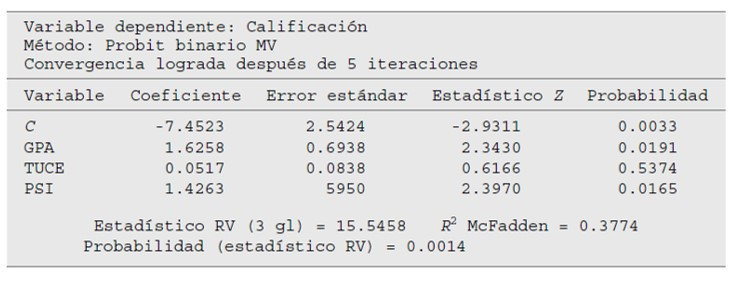
\includegraphics[width=0.8\textwidth]{9_7.JPG}
\end{center}
\end{figure}


El comando para estimar un modelo probit en Stata es \textbf{probit}


\end{frame}

%%%%%%%%%%%%%%%%%%%%%%%%%%%%%%%%%%%%%%%%%%%%%%%%%%%%%%%%%%%%

\section{¿Probit o Logit?}
\begin{frame}
\frametitle{¿Probit o Logit?}

Aunque para el ejemplo de las calificaciones los modelos logit, probit y MLP dan cualitativamente resultados semejantes, nos centraremos en los modelos logit y probit, en vista de los problemas con el MLP ya mencionados. \\

\vspace{4mm}

\highlighton{De los modelos logit y probit, ¿cuál preferiría?\\}

\vspace{4mm}

Para la mayoría de las aplicaciones, los modelos son muy semejantes; En la práctica, muchos investigadores eligen el modelo logit debido a su comparativa simplicidad matemática.

\end{frame}

%%%%%%%%%%%%%%%%%%%%%%%%%%%%%%%%%%%%%%%%%%%%%%%%%%%%%%%%%%%%




\section{Predicciones correctas}
\begin{frame}
\frametitle{Predicciones correctas}

Una forma sencilla de valorar el ajuste de un modelo de elección binaria consiste en comparar las predicciones del modelo con las respuestas observadas en la muestra.  \\

\vspace{4mm}

Para cada observación se predice la probabilidad y se asigna la respuesta de ese elemento a valores o , según la probabilidad supere o no un determinado umbral. Normalmente, el criterio de asignación emplea como punto de corte una probabilidad igual a 0,5

\begin{equation}
P(\hat{Y}_i = 1 | X) \geq 0.5  \longrightarrow \hat{Y}_i = 1
\end{equation}

\begin{equation}
P(\hat{Y}_i = 1 | X) < 0.5  \longrightarrow \hat{Y}_i = 0
\end{equation}



\end{frame}

%%%%%%%%%%%%%%%%%%%%%%%%%%%%%%%%%%%%%%%%%%%%%%%%%%%%%%%%%%%%


\section{HL}
\begin{frame}
\frametitle{Hosmer-Lemeshow}


La prueba de Hosmer-Lemeshow es otro método para estudiar la bondad de ajuste del modelo de regresión logística que consiste en comparar los valores previstos (esperados) por el modelo con los valores realmente
observados. Ambas distribuciones, esperada y observada, se contrastan mediante una prueba de $\chi^2$.

La hipótesis nula del test de Hosmer-Lemeshow es que no hay diferencias entre los valores observados y los valores pronosticados (el rechazo este test indicaría que el modelo no está bien ajustado).




\end{frame}

%%%%%%%%%%%%%%%%%%%%%%%%%%%%%%%%%%%%%%%%%%%%%%%%%%%%%%%%%%%%


%%%%%%%%%%%%%%%%%%%%%%%%%%%%%%%%%%%%%%%%%%%%%%%%%%%%%%%%%%%%








%%%%%%%%%%%%%%%%%%%%%%%%%%%%%%%%%%%%%%%%%%%%%%%%%%%%%%%%%%%%%%%%%%%%%%%


%%%%%%%%%%%%%%%%%%%%%%%%%%%%%%%%%%%%%%%%%%%%%%%%%%%%%%%%%%%%%%%%%%%%%%%

%%%%%%%%%%%%%%%%%%%%%%%%%%%%%%%%%%%%%%%%%%%%%%%%%%%%%%%%%%%%%%%%%%%%%%%







%%%%%%%%%%%%%%%%%%%%%%%%%%%%%%%%%%%%%%%%%%%%%%%%%%%%%%%%%%%%%%%%%%%%% 




\frame{
  \vspace{2cm}
  {\huge Preguntas?}


\vspace{2.5cm}

\begin{flushright}
\highlighton{
  \usebeamerfont*{frametitle}Gracias!!},
\end{flushright}

  
  \begin{flushright}
    Jr.
    
   \structure{\footnotesize{orlando.joaqui@correounivalle.edu.co}}
  \end{flushright}
}







\end{document}
